\documentclass[10pt]{scrartcl}

\usepackage[T1]{fontenc}
\usepackage{amssymb, amsmath, amsthm}
\usepackage{geometry, graphicx, enumitem, wrapfig, fancyhdr,cancel, physics}
\usepackage[english]{babel}
\usepackage{mlmodern}
\usepackage{circuitikz}

% \usepackage{listings, xcolor}
% \definecolor{codegreen}{rgb}{0,0.6,0}
% \definecolor{codegray}{rgb}{0.5,0.5,0.5}
% \definecolor{codepurple}{rgb}{0.58,0,0.82}
% \definecolor{backcolour}{rgb}{0.95,0.95,0.92}

% \lstdefinestyle{mystyle}{
%     backgroundcolor=\color{backcolour},   
%     commentstyle=\color{codegreen},
%     keywordstyle=\color{magenta},
%     numberstyle=\tiny\color{codegray},
%     stringstyle=\color{codepurple},
%     basicstyle=\ttfamily\footnotesize,
%     breakatwhitespace=false,         
%     breaklines=true,                 
%     captionpos=b,                    
%     keepspaces=true,                 
%     numbers=left,                    
%     numbersep=5pt,                  
%     showspaces=false,                
%     showstringspaces=false,
%     showtabs=false,                  
%     tabsize=4
% }
% \lstset{style=mystyle}
\geometry{a4paper, margin=0.8in}
\pagestyle{fancy}
\lhead{PH3204 - Experiment 2}
\rhead{Debayan Sarkar \texttt{22MS002}}
\everymath{\displaystyle}
\theoremstyle{definition}
\newtheorem{exercise}{Question}
\newenvironment{solution} {\begin{proof}[\normalfont \textbf{Solution}]} {\end{proof}}

\renewcommand{\qedsymbol}{}
\newcommand{\nn}{\mathbb{N}}
\newcommand{\npixL}{\frac{n\pi x}{L}}
\newcommand{\rn}{\mathbb{R}}
\newcommand{\q}{\mathbb{Q}}
\newcommand{\p}{\mathcal{P}}
\newcommand{\z}{\mathbb{Z}}
\newcommand{\dx}{\mathrm{d}x}
\newcommand*{\OO}{\hat{O}}
\newcommand*{\Op}{\hat{p}}
\newcommand*{\Ox}{\hat{x}}
\newcommand*{\OH}{\hat{H}}
\newcommand*{\Oa}{\hat{a}}
\title{Study of the characteristics of an NPN Bipolar Junction Transistor}  
\subtitle{PH3204 - Electronics Laboratory}
\author{Debayan Sarkar \\ \texttt{22MS002} \\ \texttt{Group B-10}}
\date{\today}

\geometry{a4paper, margin=1in}
\setlength{\parindent}{0pt}
\begin{document}
\maketitle
\section{Aim}
In this experiment we study the characteristics of an n-p-n bipolar junction transistor (BJT).
\section{Theory and Experimental Setup}
\subsection{NPN Bipolar Junction Transistor}
Bipolar Junction Transistors (BJTs) are utilized in circuits as switches and for signal amplification.
BJT comes in two varieties: npn and pnp. The npn BJT will be the subject of this experiment. The emitter, base, and collector are the three semiconductor layers that make up the npn BJT.
The base is lightly doped, the collector is moderately doped, and the emitter is strongly doped. The emitter-base junction and the collector-base junction are the two junctions found in the BJT.
We will examine the BJT in the Common Emitter (CE) configuration, while it can be utilized in a variety of other setups. In this setup, the base receives the input, while the collector receives the output.

\begin{figure}[!h]
    \centering
    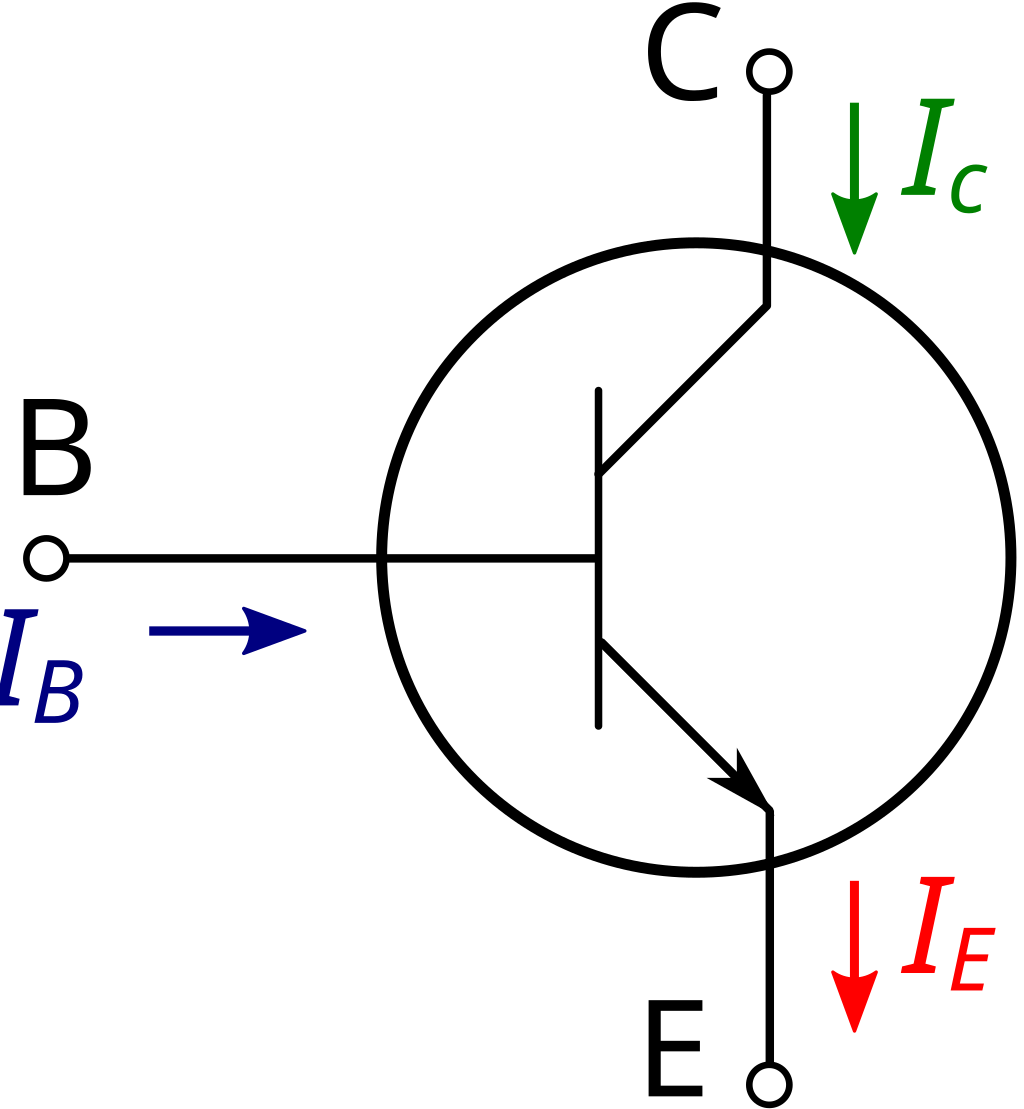
\includegraphics[width=0.3\linewidth]{BJT.png}
    \caption{NPN Bipolar Junction Transistor (Souce: The Internet)}
\end{figure}

Both the input and the output share the emitter. The plot of the base current ($I_b$) against the base-emitter voltage ($V_{BE}$) for a fixed collector voltage ($V_{CC}$) is the BJT's input characteristics.
The plot of the collector current ($I_c$) against the collector-emitter voltage ($V_{CE}$) for a fixed base current ($I_b$) represents the BJT's output characteristics.

In this experiment We also examine the BJT's current gain. The collector base junction is reverse biased and the base emitter junction is forward biased when the BJT is utilized as an amplifier. The electrons move from the emitter to the base in a forward bias and from the base to the collector in a reverse bias. The base current Ib is created by a tiny bit of recombination in the base area. The collector current $I_c$, which is determined by the following formula, is nearly equal to $I_E$:
$$I_c = \alpha I_E$$
with $\alpha \approx 1$. The current gain of the BJT is given by the formula:
$$\beta  = \cfrac{I_c}{I_b}$$
where $\beta = \cfrac{\alpha}{1 - \alpha}$ which could be quite large.
% \clearpage
\subsection{Experimental Setup}
The circuit for this experiment was prepared on a breadboard.
Below is the Circuit Diagram for the setup used in this experiment.

\begin{figure}[h!]
	\centering
	\resizebox{0.75\textwidth}{!}{
    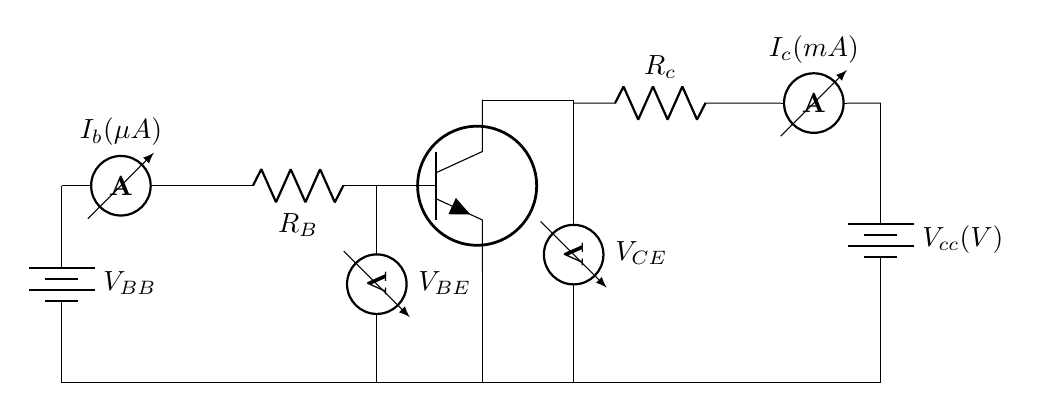
\begin{tikzpicture}
        
        % Paths, nodes and wires:
        \draw node[npn, xscale=1.41, yscale=1.41] at (8.84, 5.25) {};
        \draw (8, 5.25) to[american resistor, l={$R_B$}, label distance=0.02cm] (5, 5.25);
        \draw (3.5, 5.25) to[battery, l={$V_{BB}$}, label distance=0.02cm] (3.5, 2.75);
        \draw (7.5, 5.25) to[voltmeter, l={$V_{BE}$}, label distance=0.02cm] (7.5, 2.75);
        \draw (10, 6) to[voltmeter, l={$V_{CE}$}, label distance=0.02cm] (10, 2.75);
        \draw (8.84, 6.336) -| (10, 6);
        \draw (8.84, 4.164) |- (10, 2.75) -- (5, 2.75) |- (3.5, 2.75);
        \draw (3.5, 5.25) to[ammeter, l={$I_b(\mu A)$}, label distance=0.02cm] (5, 5.25);
        \draw (12.2, 6.3) to[ammeter, l={$I_c  (mA)$}, label distance=0.02cm] (13.9, 6.3);
        \draw (10, 6.3) to[american resistor, l={$R_c$}, label distance=0.02cm] (12.2, 6.3);
        \draw (13.9, 6.3) to[battery, l={$V_{cc}(V)$}, label distance=0.02cm] (13.9, 2.8);
        \draw (10, 2.75) -| (13.9, 2.8);
        \node[shape=circle, draw, line width=1pt, inner sep=0, minimum width=1.512cm] at (8.774, 5.25){};
    \end{tikzpicture}}
    \caption{Circuit diagram of an npn BJT in the common emmitter configuration}
\end{figure} 
\clearpage
\section{Data and Analysis}
The Data tables for both parts of this experiment can be found in the supplementary section.
\subsection{Input Characteristics}
In this part of the experiment, we studied the input characteristics of the given transistor. 
We fixed the collector voltage ($V_{CC}$) and then varied the base voltage ($V_{BB}$) and measured the
base current ($I_b$).
We had set $R_B = 1k\Omega$. We took datasets for $V_{CC} = 2V,~3V,~4V$

\begin{figure}[!h]
    \centering
    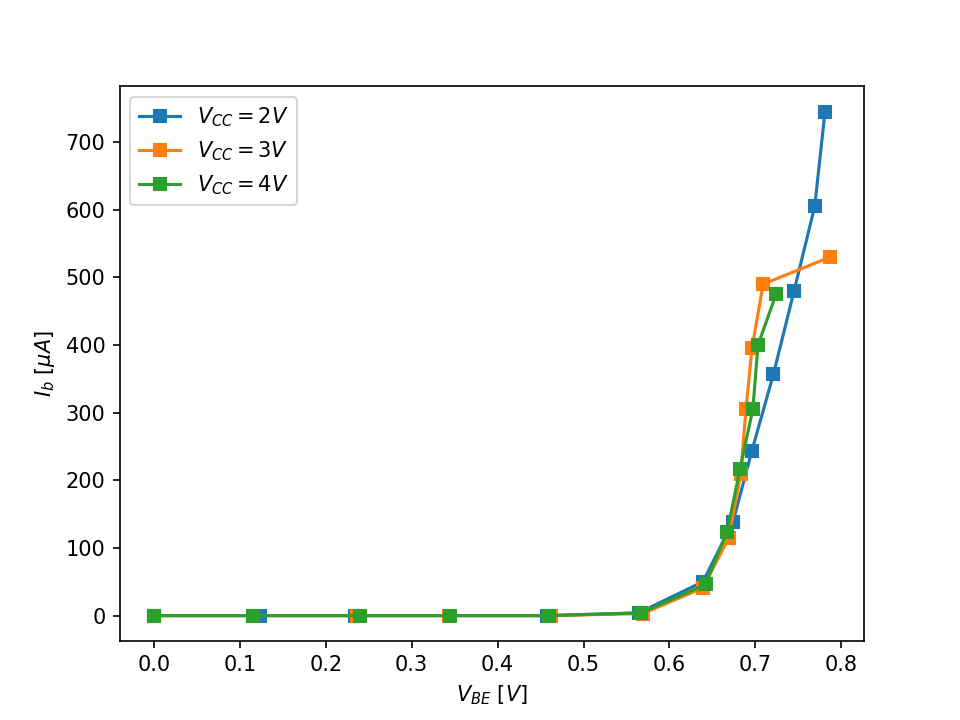
\includegraphics[width=\linewidth]{input.png}
    \caption{Input Characteristics of the given NPN BJT}
\end{figure}
The shape of the curves matches the theoretical predictions.
We expected the 2V line to be to the left of the other two, however we observed the opposite.
\clearpage
\subsection{Output Characteristics}
In this part of the experiment we studied the output characteristics of the given transistor.
We fixed the base current ($I_b$), and varied the collector-emmitter voltage ($V_{CE}$) and measured
the collector current ($I_c$). We took three datasets for $I_b = 10,~20,~30\mu A$. We had set
$R_B = 220 \Omega$ and $R_c = 1 k \Omega$.

\begin{figure}[!h]
    \centering
    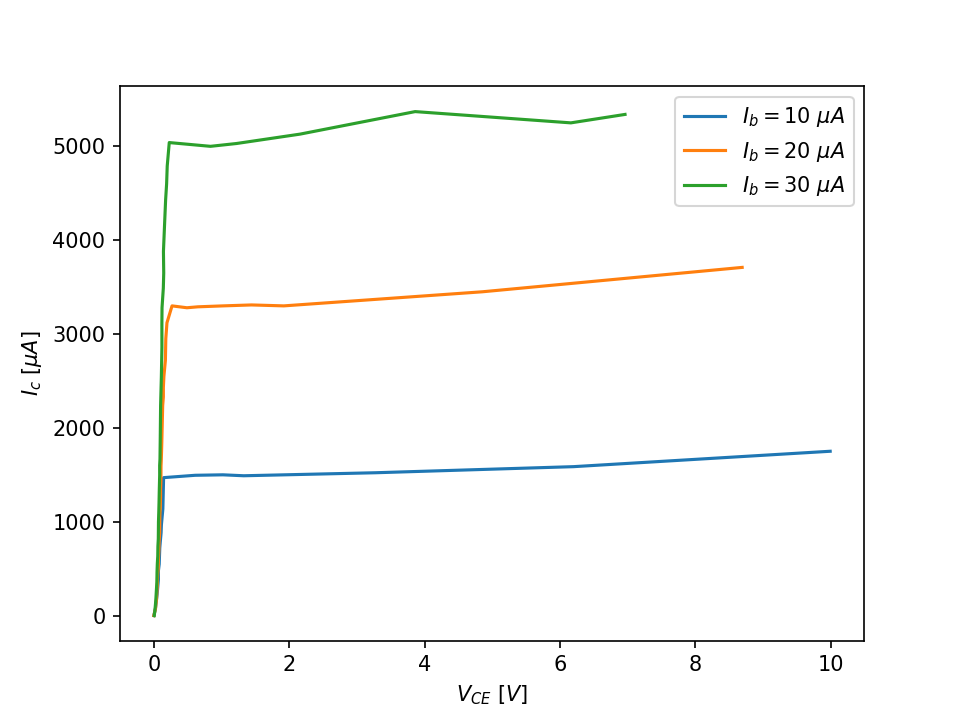
\includegraphics[width=\linewidth]{output.png}
    \caption{Output Characteristics of the given NPN BJT}
\end{figure}

As expected, the $I_b = 30 \mu A$ curve is at the top, and the $I_b = 10 \mu A$ curve is at the bottom.
Also, the shape of the curves matches the theoretical predictions.
\clearpage
\subsection{Current Gain of the BJT}
We know that the current gain of the BJT is given by the formula:
$$\beta = \cfrac{I_c}{I_b}$$
To get the Current gain, we plotted $I_c$ vs $I_b$ as obtained in the input characteristics part of the experiment.
Then, we took a linear fit of the data, to get the following values of $beta$ at different $V_BB$'s:
\begin{align*}
    &\beta_{2V} = 131.28 \pm 0.31\\
    &\beta_{3V} = 201.77 \pm 3.52\\
    &\beta_{4V} = 205.31 \pm 3.64
\end{align*}
As expected from the theory, $\beta$ is of the order of $10^2$, which is quite large. 
\begin{figure}[!h]
    \centering
    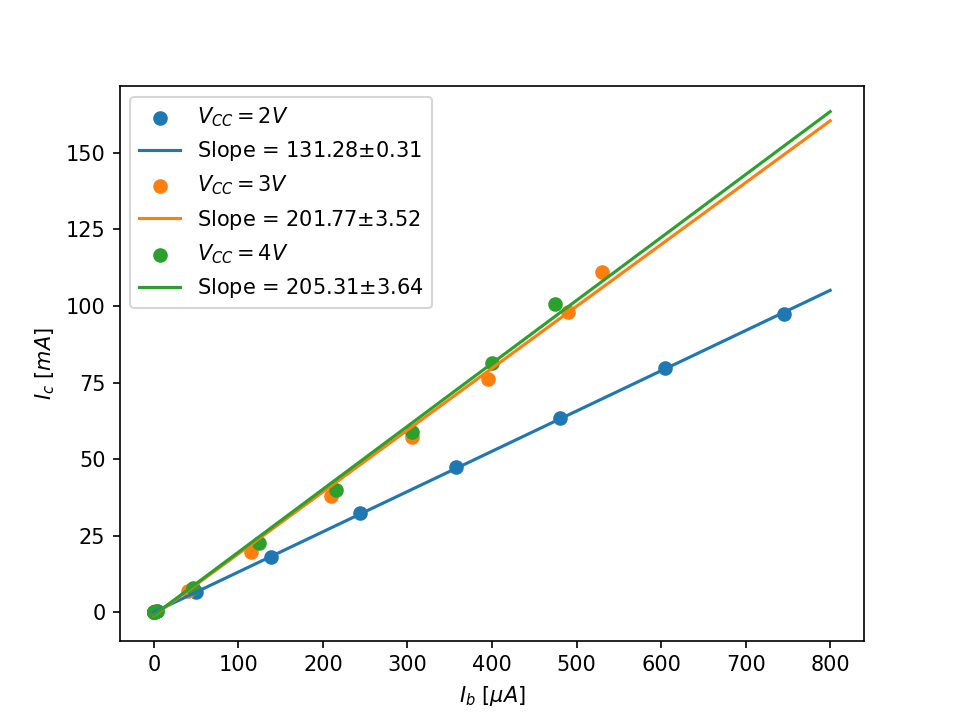
\includegraphics[width=\linewidth]{gain.png}
    \caption{Current Gain of the given NPN BJT}
\end{figure}
\clearpage
\section{Conclusion}
In conclusion, in this experiment we used the given BJT in Common Emmitter mode and collected the input and output characteristics of the given NPN BJT, and we also
measured the current gain of the transistor.
\section{Sources Of Error}
\begin{enumerate}
    \item The power source voltage was fluctuating, which could cause inaccuracies in the measurements.
    \item While collecting the output characteristics, the $I_b$ readings kept fluctuating, with a deviation of
        $\pm 3 \mu A$
    \item Loose Contacts between the Breadboard and the components, could lead to fluctuations in measurements.
    \item The multimeters are not ideal ammeters or voltmeters, hence the reading given by them isnt exact. Inaccucies due to
        the finite internal resistance of these devices also leads to some errors in the measurements.
    
\end{enumerate}
\section{Supplementary}
\label{sec:supplementary}
\begin{table}[!ht]
        \centering
        \begin{tabular}{|l|l|l|l|l|l|}
        \hline
            \textbf{V\_BB} & \textbf{V\_BE} & \textbf{I\_b (micro A)} & \textbf{I\_c( mA)} & \textbf{V\_CC} & \textbf{V\_CE} \\ \hline
            0 & 0 & 0 & 0 & 2 & 2 \\ \hline
            0.1 & 0.1232 & 0 & 0 & 2 & 2 \\ \hline
            0.2 & 0.234 & 0 & 0 & 2 & 2 \\ \hline
            0.4 & 0.458 & 0 & 0.007 & 2 & 2 \\ \hline
            0.5 & 0.564 & 4 & 0.4 & 2 & 2 \\ \hline
            0.6 & 0.639 & 50 & 6.62 & 2 & 2 \\ \hline
            0.7 & 0.674 & 139 & 18.23 & 2 & 2 \\ \hline
            0.8 & 0.696 & 244 & 32.3 & 2 & 2 \\ \hline
            0.9 & 0.721 & 357 & 47.4 & 2 & 2 \\ \hline
            1 & 0.745 & 480 & 63.4 & 2 & 2 \\ \hline
            1.1 & 0.769 & 605 & 79.6 & 2 & 2 \\ \hline
            1.2 & 0.781 & 745 & 97.3 & 2 & 2 \\ \hline
        \end{tabular}
        \caption{BJT Input Characteristics at $V_{CC} = 2V$}
        \label{tab:input2v}
    \end{table}

    \begin{table}[!ht]
        \centering
        \begin{tabular}{|l|l|l|l|l|l|}
        \hline
            \textbf{V\_BB} & \textbf{V\_BE} & \textbf{I\_b (micro A)} & \textbf{I\_c( mA)} & \textbf{V\_CC} & \textbf{V\_CE} \\ \hline
            0 & 0 & 0 & 0 & 3 & 3 \\ \hline
            0.1 & 0.1156 & 0 & 0 & 3 & 3 \\ \hline
            0.2 & 0.236 & 0 & 0 & 3 & 3 \\ \hline
            0.3 & 0.343 & 0 & 0 & 3 & 3 \\ \hline
            0.4 & 0.462 & 0 & 6.00E-03 & 3 & 3 \\ \hline
            0.5 & 0.569 & 3 & 4.88E-01 & 3 & 3 \\ \hline
            0.6 & 0.639 & 41 & 6.95 & 3 & 3 \\ \hline
            0.7 & 0.669 & 115 & 19.86 & 3 & 3 \\ \hline
            0.8 & 0.683 & 210 & 38.1 & 3 & 3 \\ \hline
            0.9 & 0.689 & 305 & 57.1 & 3 & 3 \\ \hline
            1 & 0.696 & 395 & 76.3 & 3 & 3 \\ \hline
            1.1 & 0.709 & 490 & 98.1 & 3 & 3 \\ \hline
            1.2 & 0.787 & 530 & 111.2 & 3 & 3 \\ \hline
        \end{tabular}
        \caption{BJT Input Characteristics at $V_{CC} = 3V$}
        \label{tab:input3v}
    \end{table}

    \begin{table}[!ht]
        \centering
        \begin{tabular}{|l|l|l|l|l|l|}
        \hline
            \textbf{V\_BB} & \textbf{V\_BE} & \textbf{I\_b (micro A)} & \textbf{I\_c( mA)} & \textbf{V\_CC} & \textbf{V\_CE} \\ \hline
            0 & 0 & 0 & 0 & 4 & 4 \\ \hline
            0.1 & 0.115 & 0 & 0 & 4 & 4 \\ \hline
            0.2 & 0.24 & 0 & 0 & 4 & 4 \\ \hline
            0.3 & 0.345 & 0 & 0 & 4 & 4 \\ \hline
            0.4 & 0.46 & 0 & 0.01 & 4 & 4 \\ \hline
            0.5 & 0.567 & 4 & 0.556 & 4 & 4 \\ \hline
            0.6 & 0.642 & 46 & 8.03 & 4 & 4 \\ \hline
            0.7 & 0.667 & 124 & 22.6 & 4 & 4 \\ \hline
            0.8 & 0.682 & 216 & 40 & 4 & 4 \\ \hline
            0.9 & 0.697 & 305 & 58.8 & 4 & 4 \\ \hline
            1 & 0.703 & 400 & 81.4 & 4 & 4 \\ \hline
            1.1 & 0.724 & 475 & 100.6 & 4 & 4 \\ \hline
        \end{tabular}
        \caption{BJT Input Characteristics at $V_{CC} = 4V$}
        \label{tab:input4v}
    \end{table}

    \begin{table}[!ht]
        \centering
        \begin{tabular}{|l|l|l|l|l|}
        \hline
            \textbf{V\_BB} & \textbf{I\_b (micro A)} & \textbf{I\_c( micro A)} & \textbf{V\_CC} & \textbf{V\_CE} \\ \hline
            0.44 & 10 & 0 & 0 & 0 \\ \hline
            0.46 & 10 & 70 & 0.1 & 0.0233 \\ \hline
            0.47 & 10 & 151 & 0.2 & 0.0367 \\ \hline
            0.47 & 10 & 226 & 0.3 & 0.0489 \\ \hline
            0.48 & 10 & 305 & 0.4 & 0.0584 \\ \hline
            0.5 & 10 & 385 & 0.5 & 0.0682 \\ \hline
            0.49 & 10 & 477 & 0.6 & 0.0677 \\ \hline
            0.49 & 10 & 549 & 0.7 & 0.0798 \\ \hline
            0.49 & 10 & 635 & 0.8 & 0.0837 \\ \hline
            0.49 & 10 & 720 & 0.89 & 0.0878 \\ \hline
            0.49 & 10 & 805 & 1 & 0.0978 \\ \hline
            0.5 & 10 & 882 & 1.1 & 0.1075 \\ \hline
            0.5 & 10 & 968 & 1.2 & 0.1122 \\ \hline
            0.5 & 10 & 1137 & 1.4 & 0.1335 \\ \hline
            0.51 & 10 & 1470 & 1.8 & 0.1444 \\ \hline
            0.51 & 10 & 1495 & 2.3 & 0.611 \\ \hline
            0.51 & 10 & 1.50E+03 & 2.7 & 1.021 \\ \hline
            0.51 & 10 & 1.49E+03 & 3 & 1.328 \\ \hline
            0.5 & 10 & 1522 & 4.98 & 3.27 \\ \hline
            0.5 & 10 & 1587 & 8 & 6.2 \\ \hline
            0.5 & 10 & 1751 & 11.97 & 9.99 \\ \hline
        \end{tabular}
        \caption{BJT Output Characteristics at $I_b$ = 10 $\mu A$}
        \label{tab:output10}
    \end{table}
    \begin{table}[!ht]
        \centering
        \begin{tabular}{|l|l|l|l|l|}
        \hline
            \textbf{V\_BB} & \textbf{I\_b (micro A)} & \textbf{I\_c( micro A)} & \textbf{V\_CC} & \textbf{V\_CE} \\ \hline
            0.47 & 20 & 0 & 0 & 0 \\ \hline
            0.49 & 20 & 72 & 0.1 & 0.0243 \\ \hline
            0.5 & 20 & 173 & 0.22 & 0.0393 \\ \hline
            0.5 & 20 & 251 & 0.31 & 0.0452 \\ \hline
            0.51 & 20 & 333 & 0.4 & 0.052 \\ \hline
            0.51 & 20 & 440 & 0.52 & 0.0562 \\ \hline
            0.52 & 20 & 508 & 0.6 & 0.0653 \\ \hline
            0.52 & 20 & 602 & 0.7 & 0.0686 \\ \hline
            0.52 & 20 & 696 & 0.8 & 0.0749 \\ \hline
            0.53 & 20 & 788 & 0.9 & 0.0781 \\ \hline
            0.53 & 20 & 878 & 1 & 0.0862 \\ \hline
            0.53 & 20 & 974 & 1.09 & 0.0876 \\ \hline
            0.53 & 20 & 1067 & 1.19 & 0.0894 \\ \hline
            0.53 & 20 & 1162 & 1.3 & 0.0955 \\ \hline
            0.53 & 20 & 1258 & 1.4 & 0.0997 \\ \hline
            0.53 & 20 & 1349 & 1.49 & 0.1004 \\ \hline
            0.53 & 20 & 1437 & 1.59 & 0.1051 \\ \hline
            0.54 & 20 & 1593 & 1.74 & 0.1063 \\ \hline
            0.54 & 20 & 1657 & 1.82 & 0.1102 \\ \hline
            0.54 & 20 & 1761 & 1.92 & 0.1146 \\ \hline
            0.54 & 20 & 1846 & 2 & 0.1179 \\ \hline
            0.54 & 20 & 1955 & 2.11 & 0.1214 \\ \hline
            0.54 & 20 & 2240 & 2.22 & 0.131 \\ \hline
            0.54 & 20 & 2330 & 2.32 & 0.141 \\ \hline
            0.54 & 20 & 2430 & 2.41 & 0.141 \\ \hline
            0.54 & 20 & 2550 & 2.52 & 0.149 \\ \hline
            0.54 & 20 & 2720 & 2.7 & 0.171 \\ \hline
            0.54 & 20 & 2950 & 2.9 & 0.177 \\ \hline
            0.54 & 20 & 3120 & 3.08 & 0.194 \\ \hline
            0.54 & 20 & 3300 & 3.33 & 0.269 \\ \hline
            0.54 & 20 & 3280 & 3.53 & 0.489 \\ \hline
            0.54 & 20 & 3290 & 3.7 & 0.65 \\ \hline
            0.54 & 20 & 3300 & 4.07 & 1.023 \\ \hline
            0.54 & 20 & 3310 & 4.5 & 1.443 \\ \hline
            0.54 & 20 & 3300 & 5 & 1.92 \\ \hline
            0.54 & 20 & 3450 & 8.05 & 4.85 \\ \hline
            0.54 & 20 & 3710 & 12.11 & 8.69 \\ \hline
        \end{tabular}
        \caption{BJT Output Characteristics at $I_b$ = 20 $\mu A$}
        \label{tab:output20}
    \end{table}

    \begin{table}[!ht]
    \centering
    \begin{tabular}{|l|l|l|l|l|}
    \hline
        \textbf{V\_BB} & \textbf{I\_b (micro A)} & \textbf{I\_c( micro A)} & \textbf{V\_CC} & \textbf{V\_CE} \\ \hline
        0.47 & 30 & 0 & 0 & 0.0069 \\ \hline
        0.48 & 30 & 87 & 0.1 & 0.0202 \\ \hline
        0.49 & 30 & 167 & 0.2 & 0.0295 \\ \hline
        0.49 & 30 & 274 & 0.31 & 0.0382 \\ \hline
        0.5 & 30 & 358 & 0.4 & 0.0451 \\ \hline
        0.51 & 30 & 459 & 0.51 & 0.0472 \\ \hline
        0.51 & 30 & 551 & 0.61 & 0.0516 \\ \hline
        0.51 & 30 & 634 & 0.7 & 0.0581 \\ \hline
        0.51 & 30 & 737 & 0.8 & 0.0603 \\ \hline
        0.51 & 30 & 818 & 0.89 & 0.0662 \\ \hline
        0.51 & 30 & 904 & 0.99 & 0.0675 \\ \hline
        0.52 & 30 & 997 & 1.08 & 0.0686 \\ \hline
        0.52 & 30 & 1108 & 1.2 & 0.0735 \\ \hline
        0.52 & 30 & 1209 & 1.3 & 0.0771 \\ \hline
        0.52 & 30 & 1319 & 1.42 & 0.0803 \\ \hline
        0.53 & 30 & 1358 & 1.47 & 0.0815 \\ \hline
        0.53 & 30 & 1499 & 1.61 & 0.0865 \\ \hline
        0.53 & 30 & 1599 & 1.71 & 0.0861 \\ \hline
        0.53 & 30 & 1669 & 1.78 & 0.0911 \\ \hline
        0.53 & 30 & 1894 & 2.02 & 0.0951 \\ \hline
        0.53 & 30 & 2240 & 2.19 & 0.1002 \\ \hline
        0.54 & 30 & 2540 & 2.48 & 0.1112 \\ \hline
        0.54 & 30 & 2860 & 2.8 & 0.1197 \\ \hline
        0.54 & 30 & 3110 & 3.04 & 0.1191 \\ \hline
        0.54 & 30 & 3280 & 3.21 & 0.1213 \\ \hline
        0.54 & 30 & 3490 & 3.42 & 0.1404 \\ \hline
        0.54 & 30 & 3650 & 3.62 & 0.1464 \\ \hline
        0.54 & 30 & 3880 & 3.79 & 0.1422 \\ \hline
        0.55 & 30 & 4180 & 4.09 & 0.1595 \\ \hline
        0.55 & 30 & 4430 & 4.33 & 0.1743 \\ \hline
        0.55 & 30 & 4600 & 4.5 & 0.189 \\ \hline
        0.55 & 30 & 4790 & 4.71 & 0.198 \\ \hline
        0.55 & 30 & 5040 & 4.94 & 0.228 \\ \hline
        0.55 & 30 & 5000 & 5.53 & 0.837 \\ \hline
        0.55 & 30 & 5030 & 5.97 & 1.221 \\ \hline
        0.55 & 30 & 5130 & 7.02 & 2.16 \\ \hline
        0.55 & 30 & 5370 & 8.96 & 3.86 \\ \hline
        0.55 & 30 & 5250 & 11.13 & 6.16 \\ \hline
        0.55 & 30 & 5340 & 11.98 & 6.96 \\ \hline
    \end{tabular}
    \caption{BJT Output Characteristics at $I_b$ = 30 $\mu A$}
    \label{tab:output30}
\end{table}
\end{document}
